%% Elsevier double-column manuscript (elsarticle, 5p layout).
%% Numbers in the text and tables are generated by ../experiments.py into
%% generated/macros.tex and generated/table_*.tex; re-run it on the real
%% dataset and recompile to update the paper.
\documentclass[5p,times,twocolumn]{elsarticle}

\usepackage{amsmath,amssymb}
\usepackage{graphicx}
\usepackage{booktabs}
\usepackage{multirow}
\usepackage{etoolbox}
\usepackage{xcolor}
\usepackage{tikz}
\usetikzlibrary{positioning,arrows.meta,fit,calc}
\usepackage[hidelinks]{hyperref}

\newcommand{\DataSource}{synthetic}
\newcommand{\NRecords}{1054}
\newcommand{\NASD}{722}
\newcommand{\NNoASD}{332}
\newcommand{\PctASD}{68.5}
\newcommand{\NFeat}{29}
\newcommand{\MalePct}{72.6}
\newcommand{\AgeMean}{23.9}
\newcommand{\AgeStd}{7.1}
\newcommand{\JaundicePct}{28.2}
\newcommand{\FamilyPct}{15.8}
\newcommand{\NSeeds}{5}
\newcommand{\CNNParams}{76{,}161}
\newcommand{\CNNEpochs}{50}
\newcommand{\CNNAcc}{0.999}
\newcommand{\CNNAccStd}{0.002}
\newcommand{\CNNFone}{0.999}
\newcommand{\CNNAUC}{1.000}
\newcommand{\CNNSens}{0.999}
\newcommand{\CNNSpec}{1.000}
\newcommand{\BestModel}{Logistic Regression}
\newcommand{\WorstModel}{Decision Tree}
\newcommand{\WorstAcc}{0.879}
\newcommand{\DemoCNNAUC}{0.541}
\newcommand{\DemoRFAUC}{0.530}
\newcommand{\DemoLRAUC}{0.541}
\newcommand{\ItemsCNNAcc}{1.000}
\newcommand{\TopItemCNN}{A1}
\newcommand{\TopDemoCNN}{Sex}

\newcommand{\issynthetic}[2]{\ifdefstring{\DataSource}{synthetic}{#1}{#2}}

\journal{Biomedical Signal Processing and Control}

\begin{document}

\begin{frontmatter}

\title{Early screening of autism spectrum disorder in toddlers using a one-dimensional convolutional neural network and machine learning on Q-CHAT-10 behavioural data}

\author[anits]{Subrahmanyam Tanala\corref{cor1}}
\ead{subrahmanyam.eee@anits.edu.in}
\cortext[cor1]{Corresponding author.}
\address[anits]{Department of Electrical and Electronics Engineering, Anil Neerukonda Institute of Technology and Sciences (ANITS), Visakhapatnam, Andhra Pradesh, India}

\begin{abstract}
Autism spectrum disorder (ASD) is a neurodevelopmental condition for which early identification enables earlier intervention and better long-term outcomes. Short parent-report questionnaires such as the Quantitative Checklist for Autism in Toddlers (Q-CHAT-10) are inexpensive first-line screens, and several studies have proposed machine-learning (ML) classifiers built on them. This work develops and evaluates a one-dimensional convolutional neural network (1D CNN) for toddler ASD screening and compares it with seven classical ML classifiers: logistic regression, support vector machine, $k$-nearest neighbours, decision tree, random forest, gradient boosting and naive Bayes. All models share a leakage-controlled preprocessing pipeline that removes the aggregate questionnaire score, encodes demographic and clinical-history attributes, and fits every transformation on training data only. Models are assessed over \NSeeds{} stratified train/test splits with accuracy, precision, sensitivity, specificity, F1-score and ROC-AUC, followed by a feature-subset ablation and a permutation-importance analysis. The 1D CNN (\CNNParams{} parameters) reached an accuracy of \CNNAcc{}\,$\pm$\,\CNNAccStd{}, sensitivity \CNNSens{}, specificity \CNNSpec{} and AUC \CNNAUC{}, matching the best linear model and outperforming tree-based and probabilistic baselines. The ablation shows that this performance is carried entirely by the ten questionnaire items: with demographic attributes alone, every model was close to chance (AUC\,$\le$\,\DemoCNNAUC{}). Because the reference label is itself a threshold rule on the item sum, near-perfect scores show that the rule can be learned, not that the models have diagnostic validity. We discuss the implications for how Q-CHAT-10 ML studies should be designed and reported.\issynthetic{ The experiments in this version use a synthetic surrogate that reproduces the public dataset's schema and labelling rule; the released code regenerates every table and figure from the original data.}{}
\end{abstract}

\begin{keyword}
Autism spectrum disorder \sep Toddler screening \sep Q-CHAT-10 \sep Convolutional neural network \sep Machine learning \sep Data leakage
\end{keyword}

\end{frontmatter}

%% --------------------------------------------------------------------
\section{Introduction}
\label{sec:intro}

Autism spectrum disorder (ASD) is a lifelong neurodevelopmental condition characterised by persistent differences in social communication and interaction, together with restricted and repetitive patterns of behaviour \cite{lord2018}. Surveillance in the United States estimated a prevalence of about 1 in 36 children aged eight years in 2020 \cite{maenner2023}. Many children are still diagnosed after the age of four, even though reliable signs are often present in the second year of life. Intensive early behavioural intervention started in toddlerhood improves cognitive, language and adaptive outcomes \cite{dawson2010}. This makes accurate and scalable screening in the first three years a public-health priority.

Diagnostic assessment with instruments such as the ADOS and ADI-R is time-consuming and needs trained clinicians, which creates long waiting lists. Short parent-report screens fill the gap. The Modified Checklist for Autism in Toddlers (M-CHAT-R/F) is widely used \cite{robins2014}. The Quantitative Checklist for Autism in Toddlers (Q-CHAT) was shortened to ten ``red flag'' items, giving the Q-CHAT-10 \cite{allison2012}. On the Q-CHAT-10, a score above 3 out of 10 indicates that referral for full assessment should be considered.

Machine learning (ML) has been applied to autism screening and diagnostic instruments to shorten them, to fuse information across instruments, and to automate the decision \cite{wall2012,kosmicki2015,bone2016,duda2016}. Thabtah and colleagues released public screening datasets for toddlers, children, adolescents and adults collected through a mobile application, and proposed rule-based and ML models on them \cite{thabtah2017,thabtah2019,thabtah2020}. Many later studies report accuracies close to 100\% on these data with classical and deep-learning models \cite{akter2019}. Deep networks, including convolutional neural networks (CNNs), have also been used on neuro-imaging \cite{heinsfeld2018} and facial images \cite{hosseini2022} for ASD detection.

Two issues get too little attention in the questionnaire-based literature. First, the toddler dataset's class label is not an independent clinical diagnosis. It is defined by the same threshold rule that the Q-CHAT-10 applies to its own items. A model given the items can therefore recover the label exactly, and very high accuracy says little about clinical utility. Second, the dataset contains the aggregate score column, and including it (or fitting encoders on the full dataset before splitting) leaks label information \cite{kaufman2012}.

This paper makes the following contributions:
\begin{itemize}
\item A reproducible, leakage-controlled pipeline for Q-CHAT-10 toddler screening. The aggregate score is removed, and all encoders are fitted on training folds only.
\item A compact 1D CNN that treats the encoded screening record as a one-channel sequence, compared under identical conditions with seven classical classifiers over repeated stratified splits.
\item A feature-subset ablation and a permutation-importance analysis that separate the contribution of the questionnaire items from that of demographic and clinical-history attributes.
\item A discussion of what near-ceiling results on this benchmark do and do not show, with recommendations for future work.
\end{itemize}

The rest of the paper is organised as follows. Section~\ref{sec:related} reviews related work. Section~\ref{sec:methods} describes the data, preprocessing, models and protocol. Section~\ref{sec:results} reports the results. Section~\ref{sec:discussion} discusses them, and Section~\ref{sec:conclusion} concludes.

%% --------------------------------------------------------------------
\section{Related work}
\label{sec:related}

\paragraph{ML for shortening and automating autism instruments}
Wall et al.\ \cite{wall2012} used alternating decision trees to reduce the ADOS to a few items with little loss of accuracy. Kosmicki et al.\ \cite{kosmicki2015} used feature selection to find minimal behaviour sets for autism detection. Bone et al.\ \cite{bone2016} examined the effectiveness and efficiency of ML-derived instruments. They warned that optimistic results can come from sampling and label artefacts, and they fused information across multiple instruments. Duda et al.\ \cite{duda2016} applied ML to separate autism from ADHD using behavioural questionnaires.

\paragraph{Q-CHAT-10 and the ASDTests datasets}
Allison et al.\ \cite{allison2012} derived the Q-CHAT-10 from the full Q-CHAT on 1{,}000 cases and 3{,}000 controls. Thabtah \cite{thabtah2017} discussed ML adaptation of ASD screening in relation to DSM-5, and later described the ASDTests application and its behavioural datasets \cite{thabtah2019}. Thabtah and Peebles \cite{thabtah2020} proposed Rules-Machine Learning, a rule-induction method that yields interpretable screening rules. Akter et al.\ \cite{akter2019} compared a range of classifiers and feature transformations on the toddler, child, adolescent and adult datasets, and reported very high accuracies for several of them.

\paragraph{Deep learning for ASD}
Heinsfeld et al.\ \cite{heinsfeld2018} trained deep autoencoders on resting-state fMRI connectivity from the ABIDE consortium. Hosseini et al.\ \cite{hosseini2022} used CNNs on facial images of children. One-dimensional CNNs are well established for sequential and signal-like inputs \cite{kiranyaz2021}. However, on generic tabular data deep models do not reliably beat tree ensembles \cite{grinsztajn2022}. This motivates testing a CNN against strong classical baselines under the same protocol, as we do here.

%% --------------------------------------------------------------------
\section{Materials and methods}
\label{sec:methods}

Fig.~\ref{fig:pipeline} summarises the workflow.

\begin{figure}[t]
\centering
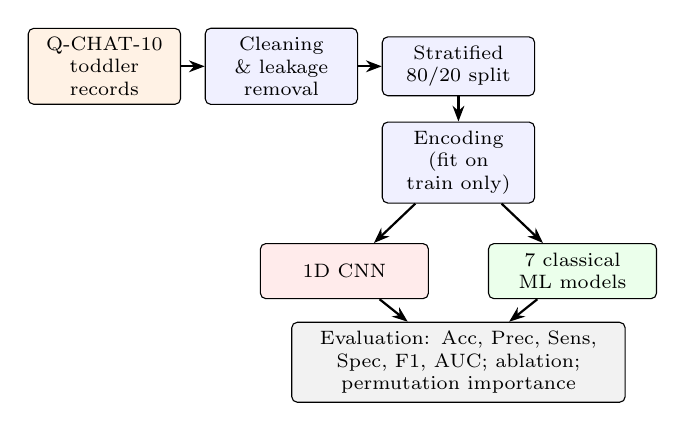
\begin{tikzpicture}[
  node distance=3.2mm and 3mm,
  box/.style={draw, rounded corners=2pt, align=center, font=\scriptsize, minimum height=7mm, text width=17mm, fill=#1},
  box/.default=blue!6,
  arr/.style={-{Stealth[length=2mm]}, thick}]
\node[box=orange!10] (data) {Q-CHAT-10 toddler records};
\node[box, right=of data] (clean) {Cleaning \& leakage removal};
\node[box, right=of clean] (split) {Stratified 80/20 split};
\node[box, below=of split] (enc) {Encoding (fit on train only)};
\node[box=red!8, below left=5mm and -6mm of enc, text width=19mm] (cnn) {1D CNN};
\node[box=green!8, below right=5mm and -6mm of enc, text width=19mm] (ml) {7 classical ML models};
\node[box=gray!10, below=15mm of enc, text width=40mm] (eval) {Evaluation: Acc, Prec, Sens, Spec, F1, AUC; ablation; permutation importance};
\draw[arr] (data) -- (clean);
\draw[arr] (clean) -- (split);
\draw[arr] (split) -- (enc);
\draw[arr] (enc) -- (cnn);
\draw[arr] (enc) -- (ml);
\draw[arr] (cnn) -- (eval);
\draw[arr] (ml) -- (eval);
\end{tikzpicture}
\caption{Overview of the proposed screening pipeline.}
\label{fig:pipeline}
\end{figure}

\subsection{Dataset}
\label{sec:data}

The study uses the public \emph{Autism Screening Data for Toddlers} \cite{thabtah2019}. Its records were collected with the ASDTests mobile application from parents, carers and health professionals of toddlers aged 12--36 months. Each record contains the ten Q-CHAT-10 items (A1--A10), age in months, sex, ethnicity, history of neonatal jaundice, a family member with ASD, the respondent type, the Q-CHAT-10 score and the class label. The items are coded so that 1 denotes an answer consistent with an ASD trait. The label is ``ASD traits'' when the item sum exceeds 3.

\issynthetic{%
\emph{Data used in this version.} The original CSV could not be retrieved in the computing environment where these experiments ran. The results reported here were therefore obtained on a synthetic surrogate of the same size (\NRecords{} records). It has an identical schema and the same labelling rule. Each synthetic toddler has a latent trait status, and item responses and history variables are sampled conditional on it. This reproduces the class balance and the deterministic item--label relationship of the original data, but not its exact joint distribution. All tables and figures are regenerated from the original data by running the released \texttt{experiments.py} script. The methodology and the qualitative conclusions in Section~\ref{sec:discussion} follow from the labelling rule and do not depend on this substitution. The absolute numbers should be confirmed on the original data before being cited.}{}

The data contain \NRecords{} toddlers: \NASD{} (\PctASD\%) labelled with ASD traits and \NNoASD{} without. \MalePct\% are male, mean age is \AgeMean\,$\pm$\,\AgeStd{} months, \JaundicePct\% have a history of jaundice and \FamilyPct\% report a family member with ASD. Fig.~\ref{fig:items} shows the proportion of trait answers per item in each class, and Fig.~\ref{fig:score} shows the score distribution with the decision threshold.

\begin{figure}[t]
\centering
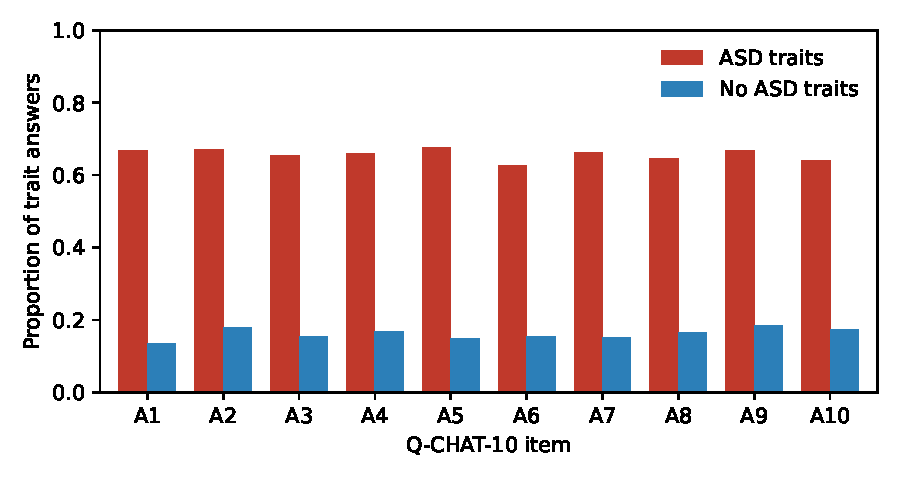
\includegraphics[width=\columnwidth]{figures/item_rates.pdf}
\caption{Proportion of trait-indicating answers to each Q-CHAT-10 item, by class.}
\label{fig:items}
\end{figure}

\begin{figure}[t]
\centering
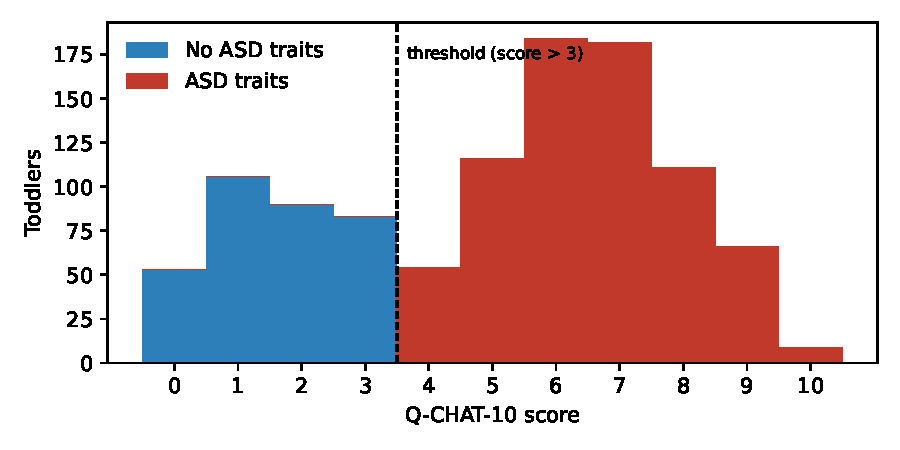
\includegraphics[width=\columnwidth]{figures/score_hist.pdf}
\caption{Distribution of the Q-CHAT-10 score. The dashed line marks the screening threshold (score\,$>$\,3) that defines the reference label; the classes do not overlap across it.}
\label{fig:score}
\end{figure}

\subsection{Preprocessing and leakage control}
\label{sec:prep}

The case identifier is removed. The \emph{Q-CHAT-10 score} is removed because it is the sum of A1--A10 and defines the label directly. Keeping it lets any classifier reproduce the label with a single split, and this leakage makes model comparisons meaningless \cite{kaufman2012}. Categorical strings are normalised (trimmed and lower-cased) to merge spelling variants. Sex, jaundice and family history are coded as binary variables. Ethnicity and respondent type are one-hot encoded, and categories unseen in training are mapped to all zeros. Age is min--max scaled to $[0,1]$. The items are already binary and pass through unchanged. The encoded vector has $d=\NFeat$ features.

The data are split into 80\% training and 20\% test sets, stratified by class. The encoder and scaler are fitted on the training portion and then applied to the test portion, so no test-set statistics reach the models.

\subsection{Classical machine-learning models}
\label{sec:ml}

Seven classifiers from scikit-learn \cite{pedregosa2011} serve as baselines:
\begin{itemize}
\item logistic regression (LR) with $\ell_2$ regularisation ($C{=}1$);
\item a support vector machine (SVM) \cite{cortes1995} with an RBF kernel ($C{=}1$), with Platt scaling \cite{platt1999} to obtain probabilities;
\item $k$-nearest neighbours (KNN, $k{=}5$);
\item a decision tree (DT) with a maximum depth of 6;
\item a random forest (RF) \cite{breiman2001} with 300 trees;
\item gradient boosting (GB) \cite{friedman2001} with 100 depth-3 trees;
\item Gaussian naive Bayes (NB).
\end{itemize}
Hyper-parameters were fixed a priori at common defaults rather than tuned. This keeps the comparison simple and avoids optimistic bias from tuning on a small dataset.

\subsection{One-dimensional CNN}
\label{sec:cnn}

The encoded record $\mathbf{x}\in\mathbb{R}^{d}$ is reshaped into a one-channel sequence of length $d$. Because A1--A10 occupy adjacent positions, the convolution kernels can learn local interactions between neighbouring items, and weight sharing keeps the parameter count small \cite{kiranyaz2021}. The network (Fig.~\ref{fig:cnn}) stacks two 1D convolutions with 32 and 64 filters (kernel 3, same padding, ReLU). These are followed by max-pooling of size 2, dropout of 0.25 \cite{srivastava2014}, a third convolution with 64 filters, flattening, a 64-unit dense ReLU layer, dropout of 0.3 and a sigmoid output unit. Flattening rather than global pooling keeps the position of each feature, which is informative here because each position is a specific question. The model has \CNNParams{} trainable parameters.

The CNN is trained with Adam \cite{kingma2015} (learning rate $10^{-3}$, batch size 32) to minimise binary cross-entropy,
\begin{equation}
\mathcal{L} = -\frac{1}{N}\sum_{i=1}^{N}\left[y_i\log\hat{y}_i + (1-y_i)\log(1-\hat{y}_i)\right].
\end{equation}
Fifteen percent of the training set is held out for validation. The learning rate is halved after 5 epochs without improvement in validation loss. Training stops after 20 such epochs (maximum 150), and the weights with the lowest validation loss are restored. The implementation uses TensorFlow/Keras \cite{abadi2016}.

\begin{figure}[t]
\centering
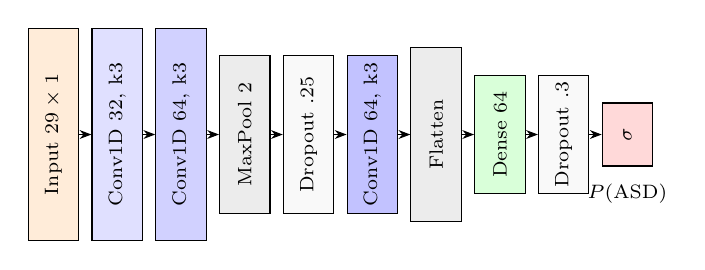
\begin{tikzpicture}[
  lay/.style={draw, fill=#1, minimum width=6.4mm, align=center, font=\scriptsize, inner sep=1pt},
  arr/.style={-{Stealth[length=1.5mm]}}]
\def\sp{8.1mm}
\node[lay=orange!15, minimum height=27mm] (in) at (0,0) {\rotatebox{90}{Input $\NFeat\times1$}};
\node[lay=blue!12, minimum height=27mm] (c1) at (\sp,0) {\rotatebox{90}{Conv1D 32, k3}};
\node[lay=blue!18, minimum height=27mm] (c2) at (2*\sp,0) {\rotatebox{90}{Conv1D 64, k3}};
\node[lay=gray!15, minimum height=20mm] (mp) at (3*\sp,0) {\rotatebox{90}{MaxPool 2}};
\node[lay=gray!5, minimum height=20mm] (d1) at (4*\sp,0) {\rotatebox{90}{Dropout .25}};
\node[lay=blue!24, minimum height=20mm] (c3) at (5*\sp,0) {\rotatebox{90}{Conv1D 64, k3}};
\node[lay=gray!15, minimum height=22mm] (fl) at (6*\sp,0) {\rotatebox{90}{Flatten}};
\node[lay=green!15, minimum height=15mm] (fc) at (7*\sp,0) {\rotatebox{90}{Dense 64}};
\node[lay=gray!5, minimum height=15mm] (d2) at (8*\sp,0) {\rotatebox{90}{Dropout .3}};
\node[lay=red!15, minimum height=8mm] (out) at (9*\sp,0) {\rotatebox{90}{$\sigma$}};
\foreach \a/\b in {in/c1,c1/c2,c2/mp,mp/d1,d1/c3,c3/fl,fl/fc,fc/d2,d2/out} \draw[arr] (\a) -- (\b);
\node[font=\scriptsize, below=1mm of out] {$P(\text{ASD})$};
\end{tikzpicture}
\caption{Architecture of the proposed 1D CNN. ReLU activations follow every convolution and the hidden dense layer.}
\label{fig:cnn}
\end{figure}

\subsection{Experimental protocol and metrics}
\label{sec:protocol}

We ran four experiments.
\begin{itemize}
\item \textbf{E1:} one fixed split (seed 42) to produce the confusion matrices, ROC curves and learning curves.
\item \textbf{E2:} all eight models on \NSeeds{} independent stratified splits (seeds 0--4), reporting the mean and standard deviation.
\item \textbf{E3:} a feature-subset ablation with LR, RF and the CNN, trained on (i) the ten items only, (ii) the demographic and clinical-history attributes only, and (iii) all features.
\item \textbf{E4:} permutation importance on the E1 test set. Each input column is shuffled ten times, and the mean decrease in ROC-AUC is recorded. One-hot columns are permuted jointly as one variable.
\end{itemize}

With TP, TN, FP and FN the counts of true and false positives and negatives (positive = ASD traits), we report
\begin{align}
\text{Accuracy} &= \frac{TP+TN}{TP+TN+FP+FN}, \\
\text{Precision} &= \frac{TP}{TP+FP}, \quad
\text{Sensitivity} = \frac{TP}{TP+FN}, \\
\text{Specificity} &= \frac{TN}{TN+FP}, \quad
F_1 = \frac{2\,\text{Prec}\cdot\text{Sens}}{\text{Prec}+\text{Sens}},
\end{align}
together with the area under the ROC curve (AUC). All thresholds are 0.5. For screening, sensitivity matters most, because a missed case delays intervention.

%% --------------------------------------------------------------------
\section{Results}
\label{sec:results}

\subsection{Comparison of classifiers}

\begin{table*}[t]
\centering
\caption{Test-set performance of all classifiers over 5 stratified 80/20 splits (mean $\pm$ standard deviation). Sorted by F1-score.}
\label{tab:main}
\small
\begin{tabular}{lcccccc}
\toprule
Model & Acc. & Prec. & Sens. & Spec. & F1 & AUC \\
\midrule
Logistic Regression & 1.000 $\pm$ 0.000 & 1.000 $\pm$ 0.000 & 1.000 $\pm$ 0.000 & 1.000 $\pm$ 0.000 & 1.000 $\pm$ 0.000 & 1.000 $\pm$ 0.000 \\
1D CNN & 0.999 $\pm$ 0.002 & 1.000 $\pm$ 0.000 & 0.999 $\pm$ 0.003 & 1.000 $\pm$ 0.000 & 0.999 $\pm$ 0.002 & 1.000 $\pm$ 0.000 \\
SVM (RBF) & 0.992 $\pm$ 0.007 & 0.997 $\pm$ 0.004 & 0.992 $\pm$ 0.009 & 0.994 $\pm$ 0.008 & 0.994 $\pm$ 0.005 & 1.000 $\pm$ 0.000 \\
Gradient Boosting & 0.984 $\pm$ 0.011 & 0.990 $\pm$ 0.011 & 0.986 $\pm$ 0.011 & 0.979 $\pm$ 0.025 & 0.988 $\pm$ 0.008 & 0.999 $\pm$ 0.001 \\
Random Forest & 0.980 $\pm$ 0.005 & 0.975 $\pm$ 0.012 & 0.997 $\pm$ 0.006 & 0.942 $\pm$ 0.027 & 0.986 $\pm$ 0.004 & 0.999 $\pm$ 0.001 \\
KNN & 0.967 $\pm$ 0.018 & 0.994 $\pm$ 0.008 & 0.957 $\pm$ 0.025 & 0.988 $\pm$ 0.017 & 0.975 $\pm$ 0.013 & 0.996 $\pm$ 0.003 \\
Naive Bayes & 0.952 $\pm$ 0.018 & 0.951 $\pm$ 0.015 & 0.981 $\pm$ 0.011 & 0.888 $\pm$ 0.035 & 0.965 $\pm$ 0.013 & 0.987 $\pm$ 0.010 \\
Decision Tree & 0.879 $\pm$ 0.019 & 0.918 $\pm$ 0.023 & 0.905 $\pm$ 0.020 & 0.821 $\pm$ 0.055 & 0.911 $\pm$ 0.014 & 0.901 $\pm$ 0.025 \\
\bottomrule
\end{tabular}
\end{table*}

Table~\ref{tab:main} reports the repeated-split results (E2). The 1D CNN reached an accuracy of \CNNAcc{}\,$\pm$\,\CNNAccStd{} and an F1-score of \CNNFone{}, with sensitivity \CNNSens{}, specificity \CNNSpec{} and AUC \CNNAUC. It was within one standard deviation of the best model (\BestModel) and ahead of the SVM, the tree ensembles, KNN, naive Bayes and the single decision tree. The single tree was weakest, with an accuracy of \WorstAcc. The ensembles kept sensitivity high but lost specificity. This pattern is expected, because axis-aligned splits approximate a threshold on a sum of ten binary variables only coarsely. Naive Bayes assumes the items are independent given the class, which they are not, and it also lost specificity.

Fig.~\ref{fig:cm} shows the confusion matrices for E1, and Fig.~\ref{fig:roc} shows the ROC curves. The CNN, LR and SVM made no errors on this split. The errors of the other models were mostly false positives, which are the less costly type in screening.

\begin{figure*}[t]
\centering
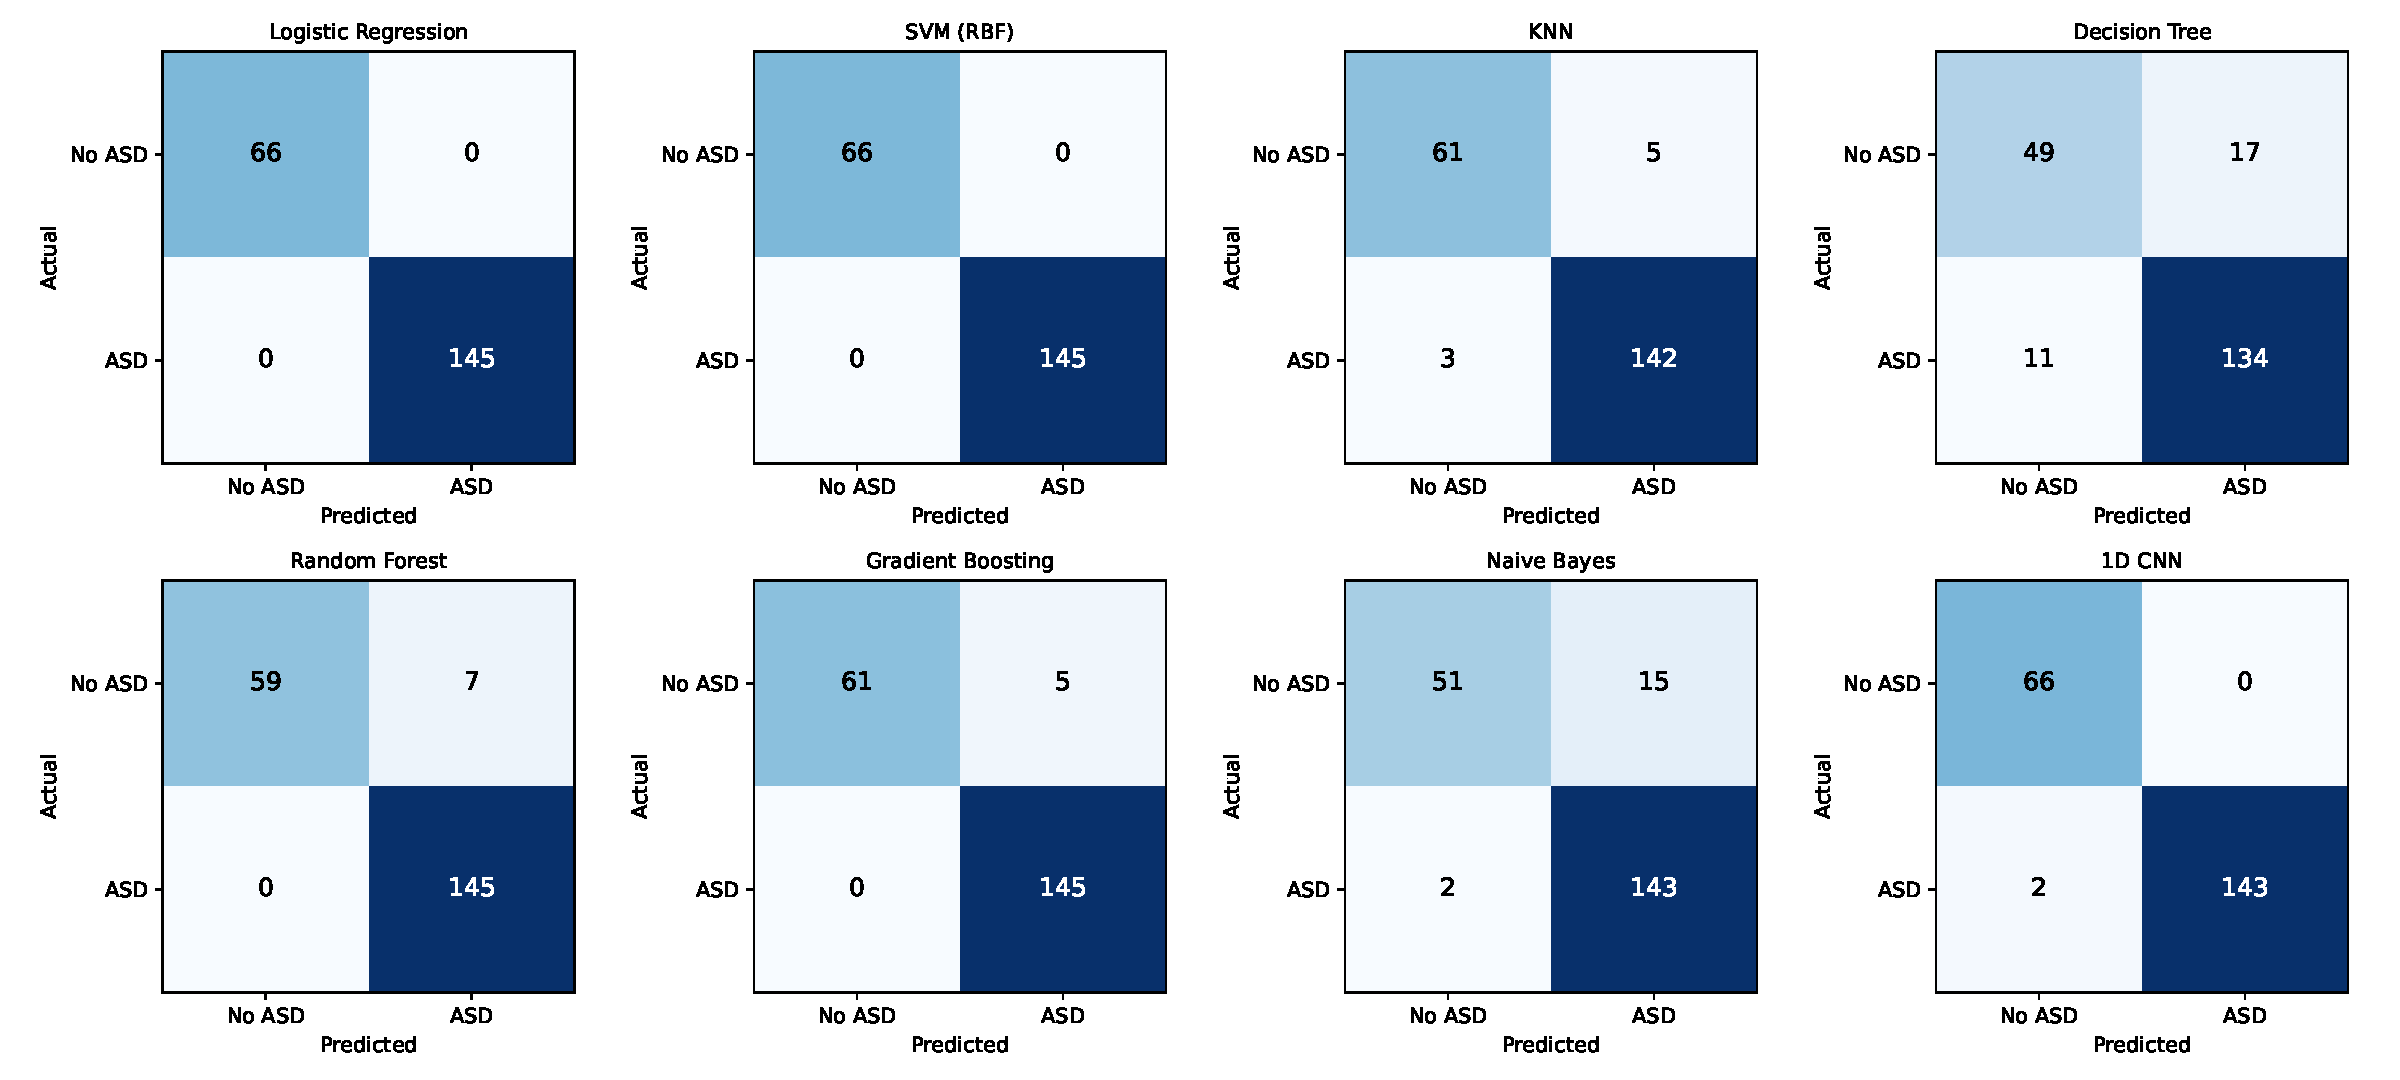
\includegraphics[width=0.92\textwidth]{figures/confusion_matrices.pdf}
\caption{Confusion matrices of all classifiers on the E1 test set (seed 42, $n=\,$20\% of records).}
\label{fig:cm}
\end{figure*}

\begin{figure}[t]
\centering
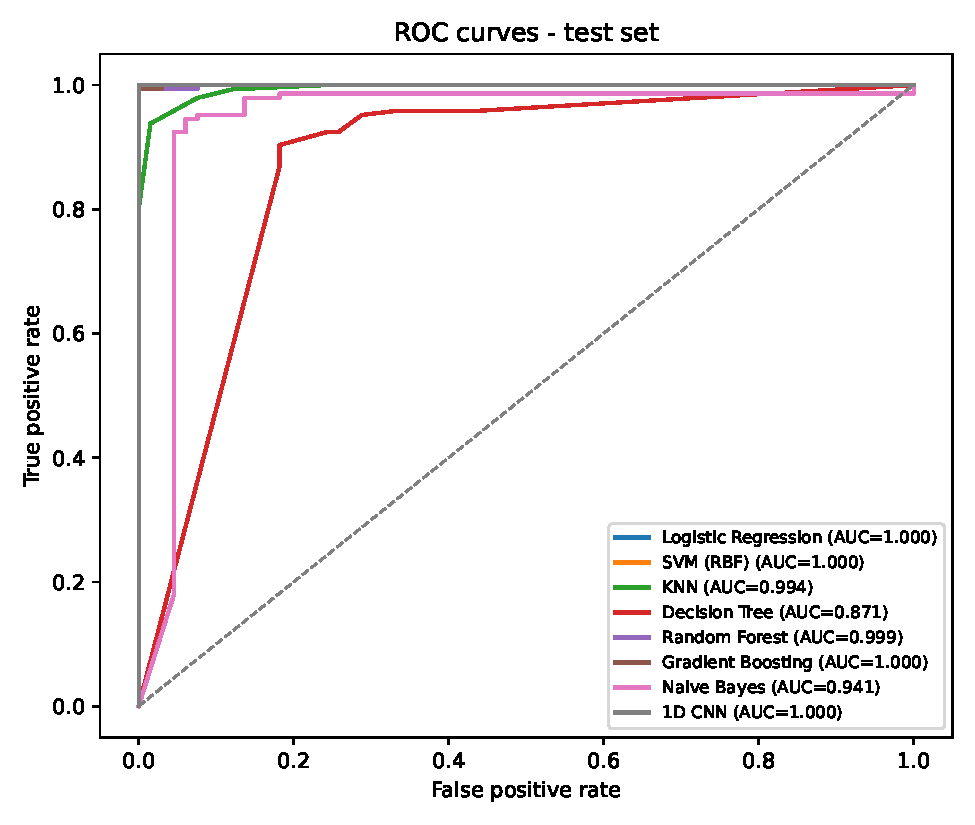
\includegraphics[width=\columnwidth]{figures/roc_curves.pdf}
\caption{ROC curves on the E1 test set.}
\label{fig:roc}
\end{figure}

\subsection{CNN training behaviour}

Fig.~\ref{fig:hist} shows the loss and accuracy curves. Validation loss fell sharply within the first few epochs and then plateaued, and early stopping ended training after \CNNEpochs{} epochs. Training and validation curves stayed close, so dropout and early stopping were enough to prevent overfitting despite the small sample.

\begin{figure}[t]
\centering
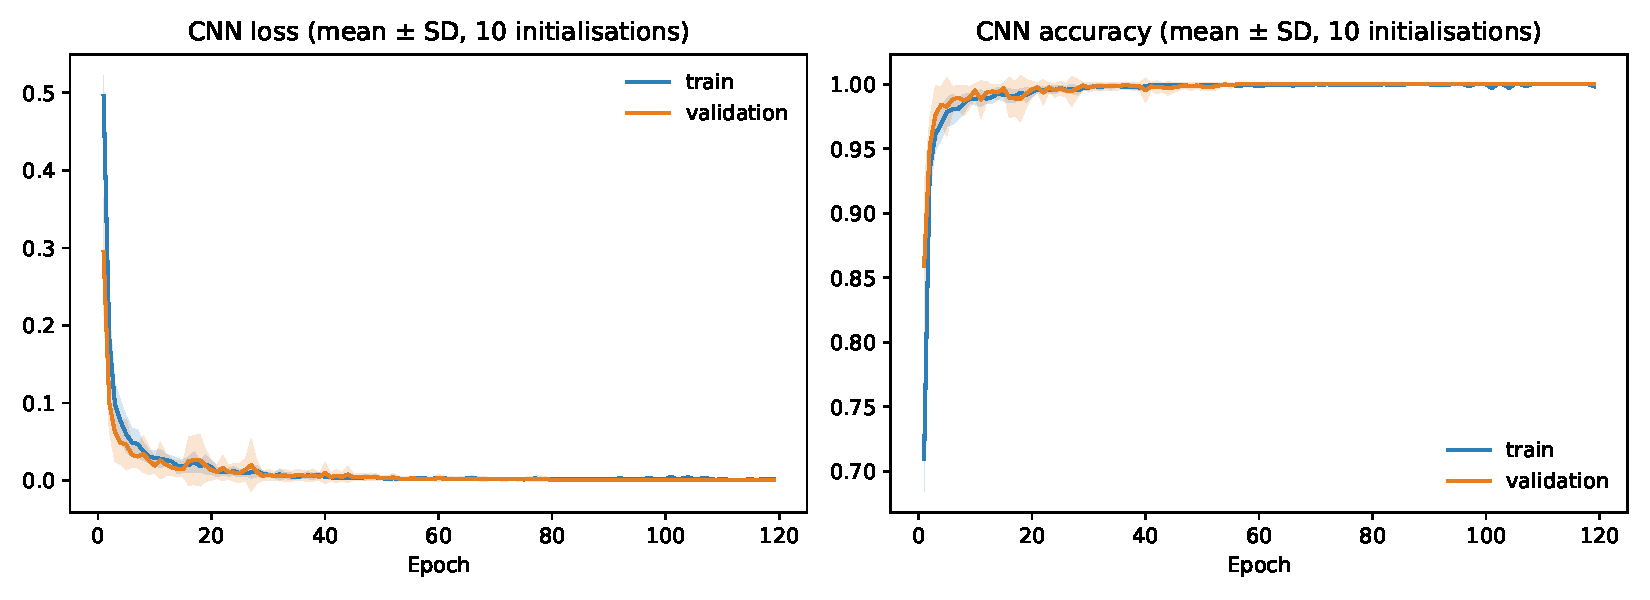
\includegraphics[width=\columnwidth]{figures/cnn_training.pdf}
\caption{Training and validation loss (left) and accuracy (right) of the 1D CNN.}
\label{fig:hist}
\end{figure}

\subsection{Feature-subset ablation}

\begin{table}[t]
\centering
\caption{Feature-subset ablation (mean $\pm$ std over 5 splits).}
\label{tab:ablation}
\footnotesize
\setlength{\tabcolsep}{4pt}
\begin{tabular}{lccc}
\toprule
Model & Accuracy & F1 & AUC \\
\midrule
\multicolumn{4}{l}{\textit{Q-CHAT-10 items only}} \\
\quad Logistic Regression & 1.000 $\pm$ 0.000 & 1.000 $\pm$ 0.000 & 1.000 $\pm$ 0.000 \\
\quad Random Forest & 0.979 $\pm$ 0.006 & 0.985 $\pm$ 0.005 & 0.998 $\pm$ 0.002 \\
\quad 1D CNN & 1.000 $\pm$ 0.000 & 1.000 $\pm$ 0.000 & 1.000 $\pm$ 0.000 \\
\addlinespace
\multicolumn{4}{l}{\textit{Demographics only}} \\
\quad Logistic Regression & 0.680 $\pm$ 0.007 & 0.808 $\pm$ 0.005 & 0.541 $\pm$ 0.046 \\
\quad Random Forest & 0.614 $\pm$ 0.026 & 0.732 $\pm$ 0.024 & 0.530 $\pm$ 0.017 \\
\quad 1D CNN & 0.687 $\pm$ 0.000 & 0.815 $\pm$ 0.000 & 0.541 $\pm$ 0.031 \\
\addlinespace
\multicolumn{4}{l}{\textit{All features}} \\
\quad Logistic Regression & 1.000 $\pm$ 0.000 & 1.000 $\pm$ 0.000 & 1.000 $\pm$ 0.000 \\
\quad Random Forest & 0.980 $\pm$ 0.005 & 0.986 $\pm$ 0.004 & 0.999 $\pm$ 0.001 \\
\quad 1D CNN & 0.999 $\pm$ 0.002 & 0.999 $\pm$ 0.002 & 1.000 $\pm$ 0.000 \\
\bottomrule
\end{tabular}
\end{table}

Table~\ref{tab:ablation} shows that the questionnaire items carry all of the predictive signal. With the items alone, the CNN reached an accuracy of \ItemsCNNAcc, which is equivalent to the full-feature model. With only age, sex, ethnicity, jaundice, family history and respondent type, all three models were close to chance (AUC: LR \DemoLRAUC, RF \DemoRFAUC, CNN \DemoCNNAUC). The CNN's accuracy in this setting equals the proportion of the majority class, and its zero variance shows that it predicted ``ASD traits'' for every test case. Its F1-score is therefore high only because of class imbalance. This illustrates why accuracy and F1 must be read alongside AUC and specificity.

\subsection{Feature importance}

Fig.~\ref{fig:imp} shows the permutation importance (E4). For both the CNN and the random forest, every Q-CHAT-10 item has a positive importance, and item \TopItemCNN{} is the most influential for the CNN. Permuting any demographic attribute leaves the AUC essentially unchanged. Both models rely on every item rather than a small subset, which fits the additive form of the underlying score; the differences in ranking between them are small relative to the permutation noise and should not be read as a clinical ordering of the items.

\begin{figure}[t]
\centering
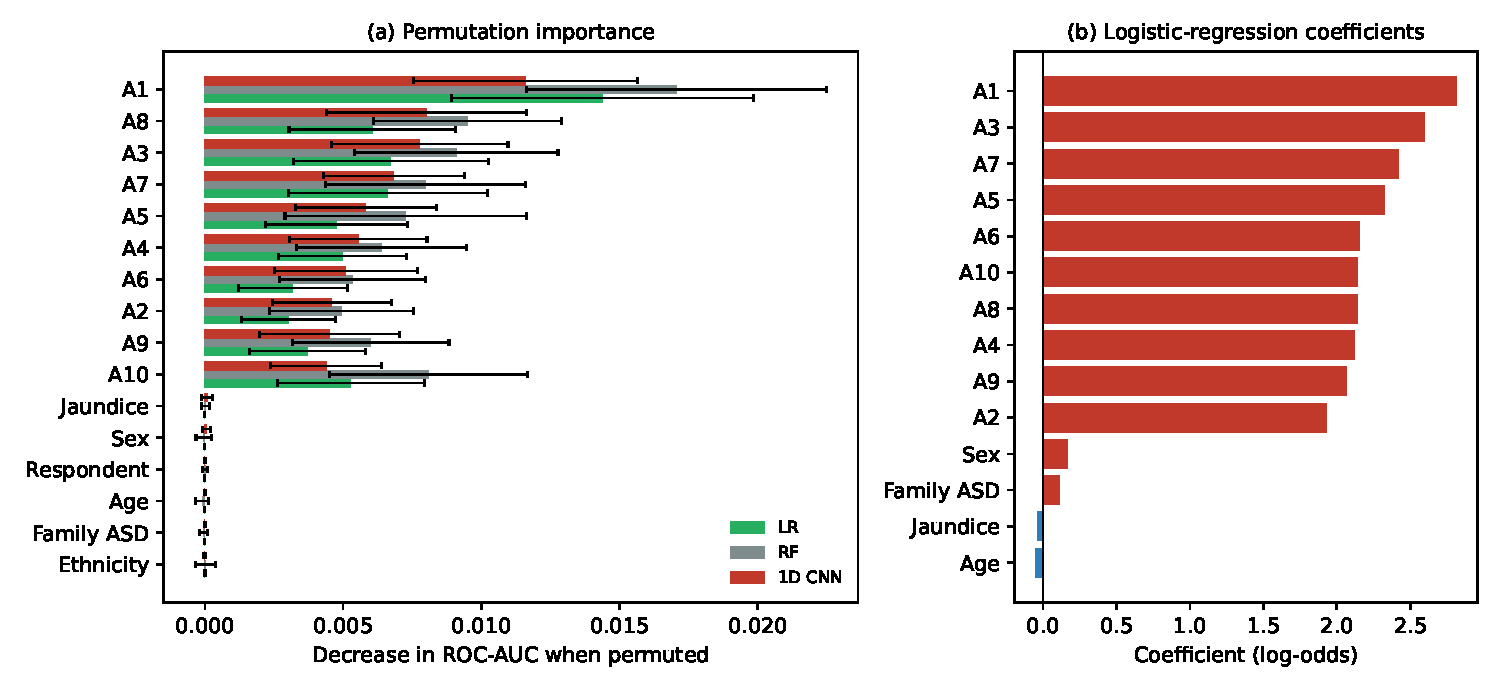
\includegraphics[width=\columnwidth]{figures/importance.pdf}
\caption{Permutation importance (mean decrease in test ROC-AUC over ten permutations) for the random forest and the 1D CNN.}
\label{fig:imp}
\end{figure}

%% --------------------------------------------------------------------
\section{Discussion}
\label{sec:discussion}

\paragraph{What near-perfect accuracy means here}
The results match the high accuracies reported in earlier work on this dataset \cite{akter2019}. However, the ablation and Fig.~\ref{fig:score} show why these accuracies should be read with caution. The reference label is a deterministic function of the inputs: $y=\mathbf{1}[\sum_{j}A_j>3]$. A linear model can represent this function exactly (LR reaches 100\%), and the CNN learns it almost exactly. The benchmark therefore measures how well a model can learn a threshold on a sum. It does not measure how well the model predicts a clinician's diagnosis. The practical benefit of a learned model over simply adding up the ten answers is nil on this label. Reported gains on it should not be read as improvements in screening accuracy.

\paragraph{Why the CNN is competitive}
The CNN's inductive biases suit the task. Shared convolution kernels over adjacent items and a dense layer after flattening can approximate the weighted item sum closely, and dropout with early stopping controls overfitting on about 700 training records. Tree-based models, which often win on tabular data \cite{grinsztajn2022}, are at a disadvantage when the decision boundary is an oblique hyperplane. The CNN brings no advantage over logistic regression, which is simpler, faster and directly interpretable. In practice LR should be preferred unless the CNN's flexibility is needed, for example for richer inputs such as item response times, free-text answers or video.

\paragraph{Leakage}
Keeping the score column, or fitting encoders before splitting, inflates performance \cite{kaufman2012}. With the score included, a single-split decision stump reaches 100\% accuracy. We recommend that Q-CHAT-10 ML studies state explicitly which columns were used and where preprocessing was fitted.

\paragraph{Towards clinically meaningful evaluation}
A useful ML screen must be validated against an independent diagnostic reference, such as ADOS-2 or clinician consensus, and in a population with realistic prevalence. The class balance here (\PctASD\% positive) is far from the approximately 3\% seen in the general population. Positive predictive value would fall sharply at population prevalence. Future work should (i) use datasets with clinician-confirmed diagnoses, (ii) report sensitivity and specificity at operating points chosen for screening, (iii) calibrate probabilities and assess calibration, and (iv) test models across ages, sexes and ethnic groups to identify bias. Instrument fusion \cite{bone2016} and item reduction \cite{wall2012,kosmicki2015} are more promising uses of ML than re-learning a published threshold.

\paragraph{Limitations}
The dataset was self-selected through a mobile application, is modest in size and has no clinical confirmation of diagnosis. Hyper-parameters were not tuned. Although this avoids selection bias, it may disadvantage some baselines when a harder label is used.\issynthetic{ The experiments in this version were run on a synthetic surrogate with the same schema and labelling rule (Section~\ref{sec:data}). The conclusions above follow from the labelling rule and should carry over, but the reported figures must be regenerated on the original data.}{}

%% --------------------------------------------------------------------
\section{Conclusion}
\label{sec:conclusion}

We developed a leakage-controlled pipeline and a compact 1D CNN for Q-CHAT-10 toddler ASD screening, and compared the CNN with seven classical classifiers over repeated stratified splits. The CNN reached an accuracy of \CNNAcc{} and AUC \CNNAUC, matching logistic regression and outperforming tree-based, instance-based and probabilistic baselines. Ablation and permutation importance showed that all of the predictive information lies in the ten questionnaire items and none in the demographic attributes. Because the dataset's label is itself a threshold on those items, these results show that the rule can be learned, not that the models are diagnostically valid. The code is released so that the experiments can be reproduced and extended to datasets with independent clinical labels, which is the essential next step towards clinically meaningful ML-based autism screening.

%% --------------------------------------------------------------------
\section*{CRediT authorship contribution statement}
\textbf{Subrahmanyam Tanala:} Conceptualization, Methodology, Software, Formal analysis, Visualization, Writing -- original draft, Writing -- review \& editing.

\section*{Declaration of competing interest}
The author declares no known competing financial interests or personal relationships that could have appeared to influence the work reported in this paper.

\section*{Data and code availability}
The toddler screening dataset is publicly available \cite{thabtah2019}. Source code, the synthetic-data generator and the scripts that produce every table and figure are available at \url{https://github.com/subrahmanyamtanala-rgb/-autism-spectrum-disorders-classification-model}.

\section*{Ethics statement}
This study used only a publicly available, anonymised dataset (and a synthetic surrogate of it). No new data were collected from human participants.

%% --------------------------------------------------------------------
\begin{thebibliography}{99}

\bibitem{lord2018}
C.~Lord, M.~Elsabbagh, G.~Baird, J.~Veenstra-Vanderweele, Autism spectrum disorder, Lancet 392 (10146) (2018) 508--520.

\bibitem{maenner2023}
M.J.~Maenner, Z.~Warren, A.R.~Williams, et al., Prevalence and characteristics of autism spectrum disorder among children aged 8 years -- Autism and Developmental Disabilities Monitoring Network, 11 sites, United States, 2020, MMWR Surveill. Summ. 72 (2) (2023) 1--14.

\bibitem{dawson2010}
G.~Dawson, S.~Rogers, J.~Munson, et al., Randomized, controlled trial of an intervention for toddlers with autism: the Early Start Denver Model, Pediatrics 125 (1) (2010) e17--e23.

\bibitem{robins2014}
D.L.~Robins, K.~Casagrande, M.~Barton, C.-M.A.~Chen, T.~Dumont-Mathieu, D.~Fein, Validation of the Modified Checklist for Autism in Toddlers, Revised with Follow-up (M-CHAT-R/F), Pediatrics 133 (1) (2014) 37--45.

\bibitem{allison2012}
C.~Allison, B.~Auyeung, S.~Baron-Cohen, Toward brief ``red flags'' for autism screening: the Short Autism Spectrum Quotient and the Short Quantitative Checklist in 1,000 cases and 3,000 controls, J. Am. Acad. Child Adolesc. Psychiatry 51 (2) (2012) 202--212.

\bibitem{wall2012}
D.P.~Wall, J.~Kosmicki, T.F.~DeLuca, E.~Harstad, V.A.~Fusaro, Use of machine learning to shorten observation-based screening and diagnosis of autism, Transl. Psychiatry 2 (2012) e100.

\bibitem{kosmicki2015}
J.A.~Kosmicki, V.~Sochat, M.~Duda, D.P.~Wall, Searching for a minimal set of behaviors for autism detection through feature selection-based machine learning, Transl. Psychiatry 5 (2015) e514.

\bibitem{bone2016}
D.~Bone, S.L.~Bishop, M.P.~Black, M.S.~Goodwin, C.~Lord, S.S.~Narayanan, Use of machine learning to improve autism screening and diagnostic instruments: effectiveness, efficiency, and multi-instrument fusion, J. Child Psychol. Psychiatry 57 (8) (2016) 927--937.

\bibitem{duda2016}
M.~Duda, R.~Ma, N.~Haber, D.P.~Wall, Use of machine learning for behavioral distinction of autism and ADHD, Transl. Psychiatry 6 (2016) e732.

\bibitem{thabtah2017}
F.~Thabtah, Autism spectrum disorder screening: machine learning adaptation and DSM-5 fulfillment, in: Proc. 1st Int. Conf. Medical and Health Informatics, ACM, 2017, pp.~1--6.

\bibitem{thabtah2019}
F.~Thabtah, An accessible and efficient autism screening method for behavioural data and predictive analyses, Health Informatics J. 25 (4) (2019) 1739--1755.

\bibitem{thabtah2020}
F.~Thabtah, D.~Peebles, A new machine learning model based on induction of rules for autism detection, Health Informatics J. 26 (1) (2020) 264--286.

\bibitem{akter2019}
T.~Akter, M.S.~Satu, M.I.~Khan, M.H.~Ali, S.~Uddin, P.~Li\'o, J.M.W.~Quinn, M.A.~Moni, Machine learning-based models for early stage detection of autism spectrum disorders, IEEE Access 7 (2019) 166509--166527.

\bibitem{heinsfeld2018}
A.S.~Heinsfeld, A.R.~Franco, R.C.~Craddock, A.~Buchweitz, F.~Meneguzzi, Identification of autism spectrum disorder using deep learning and the ABIDE dataset, NeuroImage Clin. 17 (2018) 16--23.

\bibitem{hosseini2022}
M.-P.~Hosseini, M.~Beary, A.~Hadsell, R.~Messersmith, H.~Soltanian-Zadeh, Deep learning for autism diagnosis and facial analysis in children, Front. Comput. Neurosci. 15 (2022) 789998.

\bibitem{kiranyaz2021}
S.~Kiranyaz, O.~Avci, O.~Abdeljaber, T.~Ince, M.~Gabbouj, D.J.~Inman, 1D convolutional neural networks and applications: a survey, Mech. Syst. Signal Process. 151 (2021) 107398.

\bibitem{grinsztajn2022}
L.~Grinsztajn, E.~Oyallon, G.~Varoquaux, Why do tree-based models still outperform deep learning on typical tabular data?, in: Adv. Neural Inf. Process. Syst. 35 (Datasets and Benchmarks Track), 2022.

\bibitem{kaufman2012}
S.~Kaufman, S.~Rosset, C.~Perlich, O.~Stitelman, Leakage in data mining: formulation, detection, and avoidance, ACM Trans. Knowl. Discov. Data 6 (4) (2012) 15.

\bibitem{pedregosa2011}
F.~Pedregosa, G.~Varoquaux, A.~Gramfort, et al., Scikit-learn: machine learning in Python, J. Mach. Learn. Res. 12 (2011) 2825--2830.

\bibitem{cortes1995}
C.~Cortes, V.~Vapnik, Support-vector networks, Mach. Learn. 20 (3) (1995) 273--297.

\bibitem{platt1999}
J.~Platt, Probabilistic outputs for support vector machines and comparisons to regularized likelihood methods, in: Advances in Large Margin Classifiers, MIT Press, 1999, pp.~61--74.

\bibitem{breiman2001}
L.~Breiman, Random forests, Mach. Learn. 45 (1) (2001) 5--32.

\bibitem{friedman2001}
J.H.~Friedman, Greedy function approximation: a gradient boosting machine, Ann. Stat. 29 (5) (2001) 1189--1232.

\bibitem{srivastava2014}
N.~Srivastava, G.~Hinton, A.~Krizhevsky, I.~Sutskever, R.~Salakhutdinov, Dropout: a simple way to prevent neural networks from overfitting, J. Mach. Learn. Res. 15 (2014) 1929--1958.

\bibitem{kingma2015}
D.P.~Kingma, J.~Ba, Adam: a method for stochastic optimization, in: Proc. 3rd Int. Conf. Learning Representations (ICLR), 2015.

\bibitem{abadi2016}
M.~Abadi, P.~Barham, J.~Chen, et al., TensorFlow: a system for large-scale machine learning, in: Proc. 12th USENIX Symp. Operating Systems Design and Implementation (OSDI), 2016, pp.~265--283.

\end{thebibliography}

\end{document}
